% -----------------------------------------------
% Template for FMA2014
% (based on ISMIR 2010 Template)
% -----------------------------------------------
%
% To compile run:
% pdflatex fma2014template.tex
% bibtex fma2014template
% pdflatex fma2014template.tex (probably twice)
%

\documentclass{article}
\usepackage[authoryear]{natbib}
\usepackage{fma2014}
\usepackage{amsmath}
\usepackage{graphicx}

% Title.
% ------
\title{Score-aided lyrics to audio alignment in ottoman recordings}

% Single address
% To use with only one author or several with the _same address_
% ---------------
%\oneauthor
% {Author}
% {Affiliation \\ {\tt {author}@fma.edu}}
%
\oneauthor
 {Author1, Author2}
 {Affiliation \\ {\tt \{author1,author2\}@fma.edu}}
%
% Two addresses
% --------------
%\twoauthors
%  {First author, Second Author} {Affiliation1 \\ {\tt author1@fma.edu, author2@afm.edu}}
%  {Third author} {Affiliation2 \\ {\tt author3@fma.edu}}
%
% Three addresses
% --------------
%\threeauthors
%  {First author} {Affiliation1 \\ {\tt author1@fma.edu}}
%  {Second author} {Affiliation2 \\ {\tt author2@fma.edu}}
%  {Third author} {Affiliation3 \\ {\tt author3@fma.edu}}


\begin{document}
%
\maketitle
%


\section{Motivation}
Lyrics are one of the most important musical aspects. More specifically, the lyrics of sarki tell a story from the ottoman folklore and help create impression of the song. When a performance is heard, most listeners will follow the lyrics of the main vocal melody.   
In this perspective the automatic synchronisation between lyrics and music poses a used-demanded research task. It is applicable in use cases including among others karaoke, mood detection or for the automatic generation of music videos.
Up to now, the synchronisation between lyrics and performances from the Ottoman music tradition has not been addressed. 

\subsection{Description of peculiarities of Ottoman music}
Most classical songs in the sarki form evidence clear structural parts including aranagme (instrumenta introduction), mezim (verse) and nakarat (refrain).
Describe sarki form more.

\section{Related work}
To date most of the studies of singing voice are focused on western polyphonic popular music. Most of the approaches to the automatic lyrics-to-audio alignment exploit phonetic acoustic features. 

An example such system for Japanese popular music \citep{fujihara2011lyricsynchronizer}
relies on a forced alignemnt scheme.  Since this technique was originally developed to carry the alignment between clean speech and text, accompanying instruments and non-vocal sections deteriorate the alignement accuracy. To address this [ref] performs several preprocessing steps of the vocal line: Firstly the waveform of the predominant melody is segregated from the polyphonic signal and then classified into vocal and non-vocal sections. Lastly, the alignment is run using phoneteic features extracted from the vocal-only signal.   

A diametrically different approach is to deploy external information sources. Mueller [ref] uses MIDI files, which are manually synchronised to lyrics. By perfroming mapping of timestamps between an audio recording and a MIDI version the composition, lyrics are  implicitly aligned to the audio.


\begin{itemize}
\item Meinard Mueller did some workshop on lyrics-to-audio (Sertan? reference?) 
\end{itemize}

\section{Method}
In this work we propose to combine advantages of these two approaches: We make use of a modeling scheme based on phonetic features.  Similar to [Hiromasa] we train a phonetic recognizer, where each phoneme is a assigned a hidden Markov model (HMM). 
Additionally, we utilize musical scores, in which sections are labeled. Songs are segmented into structural parts through an external module, which links sections from the score to anchors in the audio [Sertan].  
Using a Viterbi forced alignment, the system aligns in a non-linear way the extracted phonetic features to phoneme network of trained HMMs.(what is the result: timestamps)
 
Figure one gives an overview of the steps of alignemnt.


\begin{figure*}
 \centerline{\includegraphics[width=7.49cm]{Training.eps}\hskip1.5cm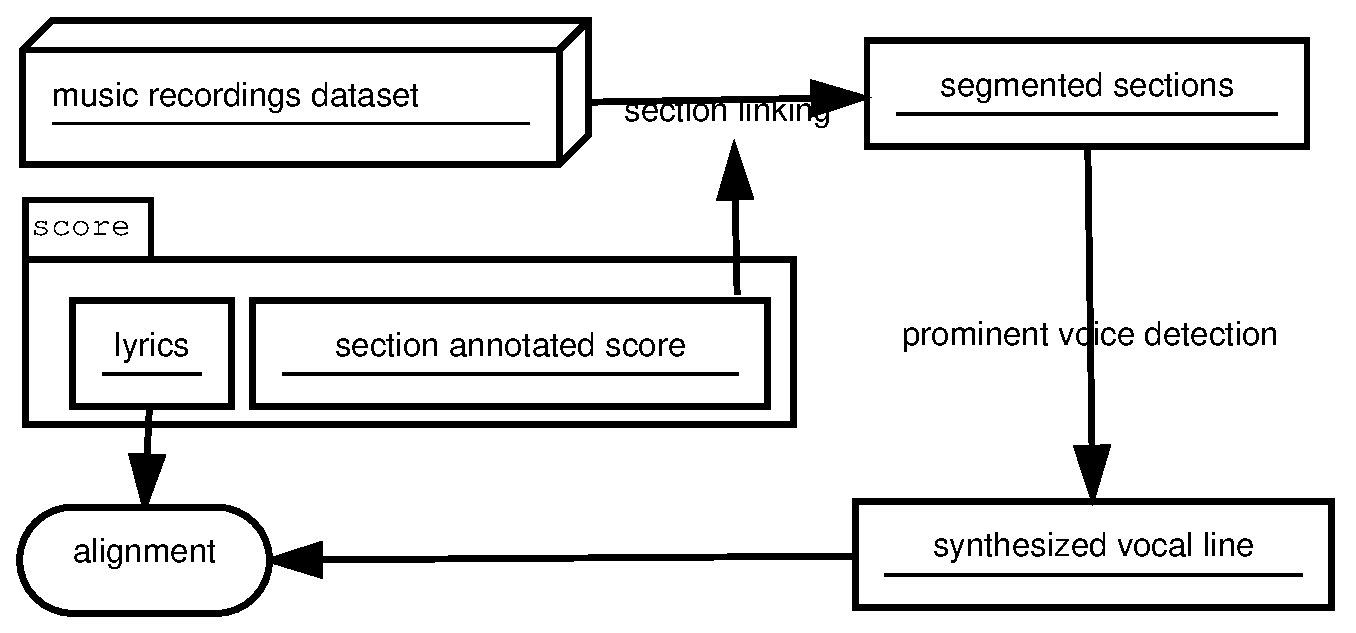
\includegraphics[width=7.49cm]{Alignment.eps}}
 \caption{Figure captions should be placed below the figure.}
 \label{fig:example}
\end{figure*}


\subsection{Training}

In the abscence of annotated data of singing phonemes, we train phoneme models on a big corpus of annotated turkish speech. Later, we adapt of speech models to match the characteristics of clean singing voice using a small singing corpus (see fig 1).

How many gaussians? and 12-component MFCCs are extracted.

\subsection{Adaptation}
Adaptation accounts for the more dynamic acoustic characteristics of sung vocals compared to speech. For example, the fluctuation of fundamental frequency (F0) and loudness for a given vocal in singing vary more than in speech sounds. 

It is an approch for speaker adaptation. The idea is to transform the acoustic space of speaker-independent phoneme models towards the acoustic characteristics of a particular speaker.  [Mesaros] has proposed instead of speaker-data to adapt the speech model to singing-voice audio using Maximum likelihood linear regression (MLLR). The MLLR transform - applied as well in this work - shifts in a linear way the mean components of the Gaussian mixtures of the speech model. This ensures that each state of the adapted HMMs is more likely to generate the corresponding state of singing audio.  

  

\subsection{Section Linking}
Research has shown that running alignment on fragmented segments of a piece leads to a more accurate results rather than running it on the whole song [ref]. Thus a necessary step to perform
alignment is the segmentation of audio into vocal-containing segments. In the sarki form each
vocal segment is associated with a section (e.g. nakarat).
A further challenge for the alignment is that typically a given performances
of a sarki tend to have repetitions of whole sections. These repetitions
are not indicated in the score. Thus for each audio recording, apriori to alignment, we utilize
an algorithm for detecting structural segments.

The method {[}ref{]} takes as input the score of a piece and an audio
recording of the same piece. (see fig 1) The scores are encoded in the machine-readable
symbTr format {[}ref{]}. The starting and ending points of the sections
are explicitly marked in the score. The method links the sections
in the score to the corresponding parts in the audio, thus creating
timestamps that mark the beginning and ending of each section segment.
% It generates a synthetic pitch contour from the score, extracts main
% pitch contour from the audio and matches the two melodic representations.

\subsection{Alignment}
To each segmented vocal section we assign the corresponding lyrical strophe automatically, because lyrics are present parallel to melody in the score. After section detection a source separation step divides the audio into singing voice and accompanying instruments.  The source separation algorithm applied is [ref]. To reduce the negative influence of accompanying instruments, MFCCs are extracted from the segregated vocal line. (Fig 1). 

The words from the lyrics are expanded to phonemes based on grapheme-to-phoneme rules for Turkish. [Table 1 of SALOR].  
Then the HMMs are concatenated into a phoneme network. An optional silent pause model, inserted at the end of each word, allows to accomodate non-vocal breaks.  These are characteristic for ends of phrases in classical turkish chants. At the end the forced alignemtn is applied. 


\section{Experimental setup}
Training of the model, adaptation and the alignment is done using the HTK.

\subsection{Data}
METU corpus. here reference to METU corpus. number of hours of speech.  


The adaptation corpus consists of 10 acapella recordings from turkish singers.  
 The adaptation data (see fig 1) is annotated on phoneme-level which allows an model reestimation in a supervised mode.
NOTE: vocals are sung with more embellishments.

\subsection{Evaluation method}		
Evaluation is done on word-level


% Reference sheet at: ftp://ftp.tex.ac.uk/tex-archive/macros/latex/contrib/natbib/natnotes.pdf

%\bibliographystyle{plainnat}
\bibliography{JabRefLyrics2Audio}

\end{document}
